\documentclass[12pt,a4paper]{article}
\usepackage[latin1]{inputenc}
\usepackage{amsmath}
\usepackage{amsfonts}
\usepackage{amssymb}
\usepackage{graphicx}
\usepackage{float}
\author{Said Zahrai}
\title{Behavioral Cloning}
\begin{document}
	\maketitle
	
	\section{Introduction}
	The goal of this project is to clone the behavior of a driver driving a car in a Unity game. A player needs to play first and record data. While the player is playing, the environment is observed with three cameras mounted in the middle of the car, and in the two left and right corners.
	\section{Data}
	\subsection{Camera recorded images}
	\begin{figure}[H]
		\centering
		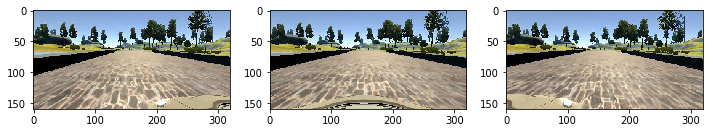
\includegraphics[width=0.7\linewidth]{writeup_figures/three_cameras_1}
		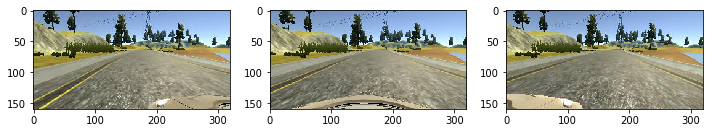
\includegraphics[width=0.7\linewidth]{writeup_figures/three_cameras_2}
		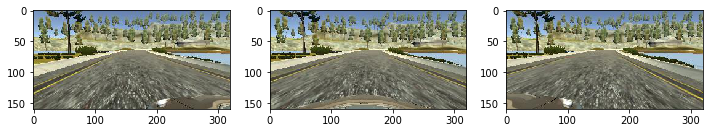
\includegraphics[width=0.7\linewidth]{writeup_figures/three_cameras_3}
		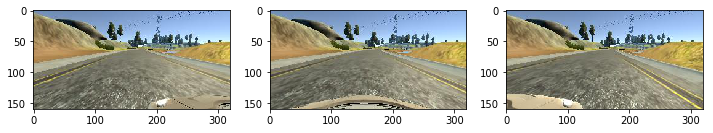
\includegraphics[width=0.7\linewidth]{writeup_figures/three_cameras_4}
		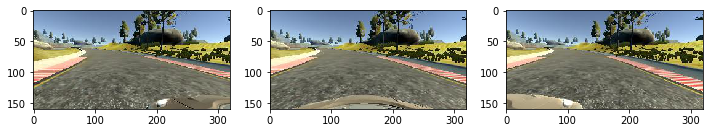
\includegraphics[width=0.7\linewidth]{writeup_figures/three_cameras_5}
		\caption{Camera recorded images. Left, seen from left camera, center from center camera and right from right camera.}
		\label{fig:threecameras}
	\end{figure}

	\begin{figure}[H]
		\centering
		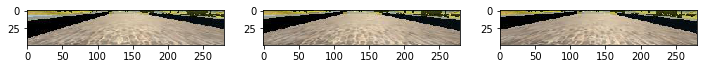
\includegraphics[width=0.7\linewidth]{writeup_figures/corped_image_1}
		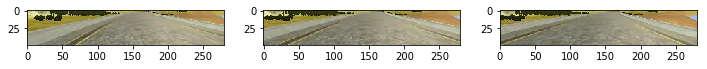
\includegraphics[width=0.7\linewidth]{writeup_figures/corped_image_2}
		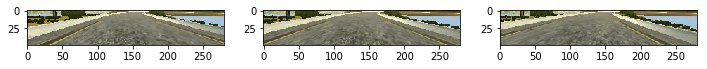
\includegraphics[width=0.7\linewidth]{writeup_figures/corped_image_3}
		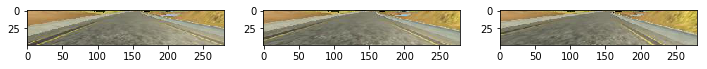
\includegraphics[width=0.7\linewidth]{writeup_figures/corped_image_4}
		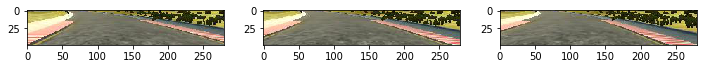
\includegraphics[width=0.7\linewidth]{writeup_figures/corped_image_5}
		\caption{Corped images with focus on interesting region. Left, seen from left camera, center from center camera and right from right camera.}
		\label{fig:corpedimages}
	\end{figure}

	\begin{figure}[H]
		\centering
		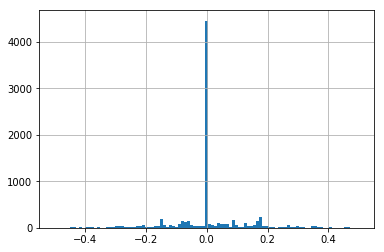
\includegraphics[width=0.7\linewidth]{writeup_figures/steering_distribution}
		\caption{Distribution of steering values.}
		\label{fig:distribution}
	\end{figure}

	\begin{figure}[H]
		\centering
		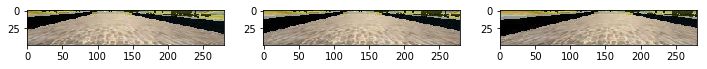
\includegraphics[width=0.7\linewidth]{writeup_figures/shifted_image_1}
		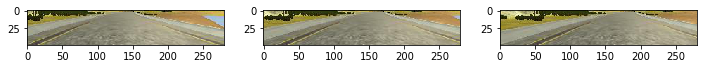
\includegraphics[width=0.7\linewidth]{writeup_figures/shifted_image_2}
		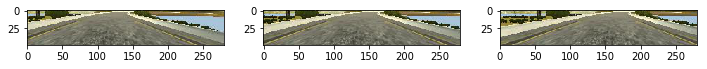
\includegraphics[width=0.7\linewidth]{writeup_figures/shifted_image_3}
		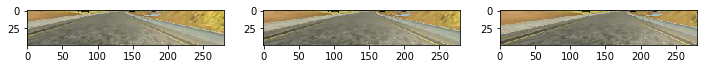
\includegraphics[width=0.7\linewidth]{writeup_figures/shifted_image_4}
		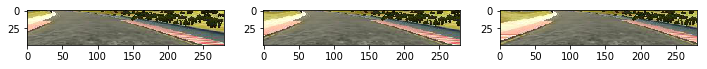
\includegraphics[width=0.7\linewidth]{writeup_figures/shifted_image_5}
		\caption{Shifted images: Left, shifted 20 pixels to left, center, original image and right, shifted 20 pixels to right.}
		\label{fig:shiftedimages}
	\end{figure}

	\subsection{Data augmentation}
	
	\texttt{img = plt.imread(image\_file\_address) \newline
		if (abs(batch\_sample[1])<0.01):\newline
		\hspace*{0.5cm} r = random.randint(0,400)\newline
		\hspace*{0.5cm} if (r<20):\newline
		\hspace*{1.0cm} images.append(img)\newline
		\hspace*{1.0cm} angles.append(steering\_value)\newline
		\hspace*{1.0cm} images.append(np.fliplr(img))\newline
		\hspace*{1.0cm} angles.append(-steering\_value)\newline
		\hspace*{0.5cm} elif (data\_augmentation):\newline
		\hspace*{1.0cm} r =random.randint(-40,40)\newline
		\hspace*{1.0cm} 
		\hspace*{1.0cm} if (abs(r)<21):\newline
		\hspace*{1.5cm} M = np.float32([[1,0, r],[0,1,0]])\newline
		\hspace*{1.5cm}  images.append(cv2.warpAffine(img,M,(cols,rows)))\newline
		\hspace*{1.5cm} angles.append(steering\_value+0.01*r)}
	
	
	\begin{figure}[H]
		\centering
		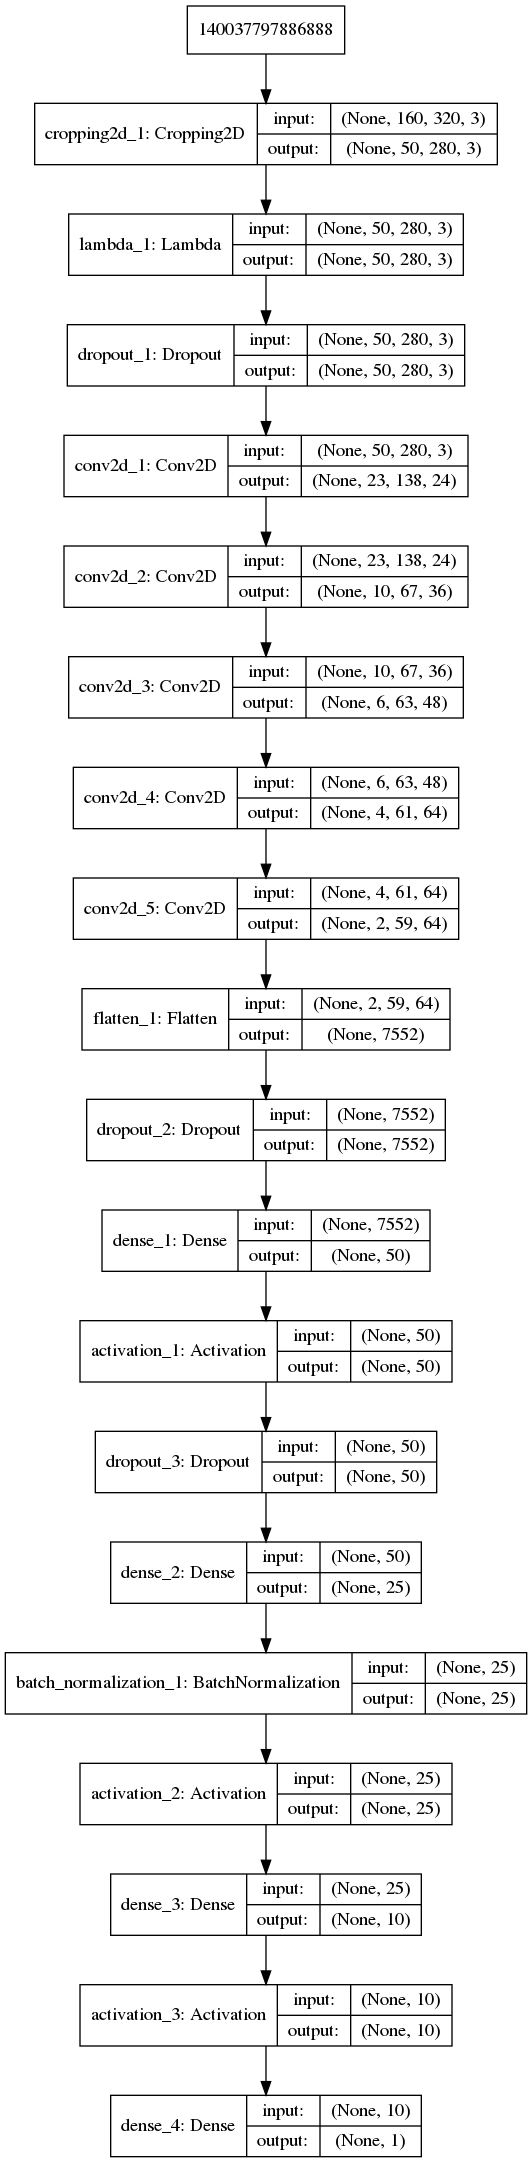
\includegraphics[width=0.3\linewidth]{writeup_figures/nvidia_model_structure}
		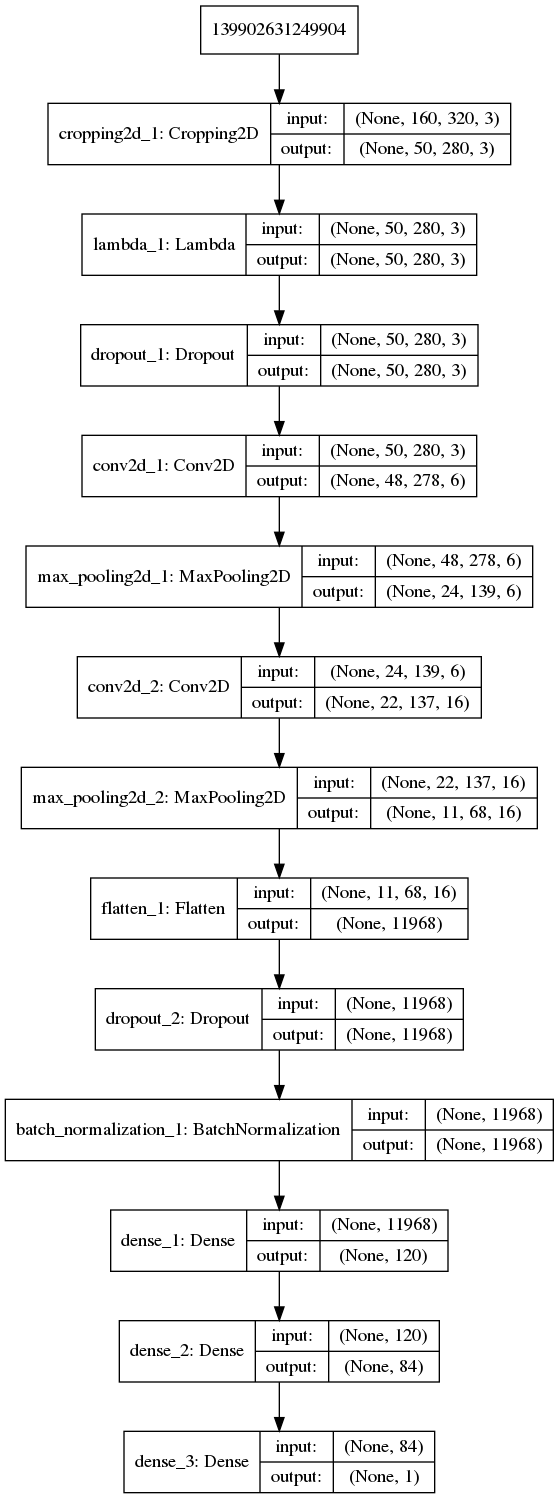
\includegraphics[width=0.3\linewidth]{writeup_figures/lenet_model_structure}		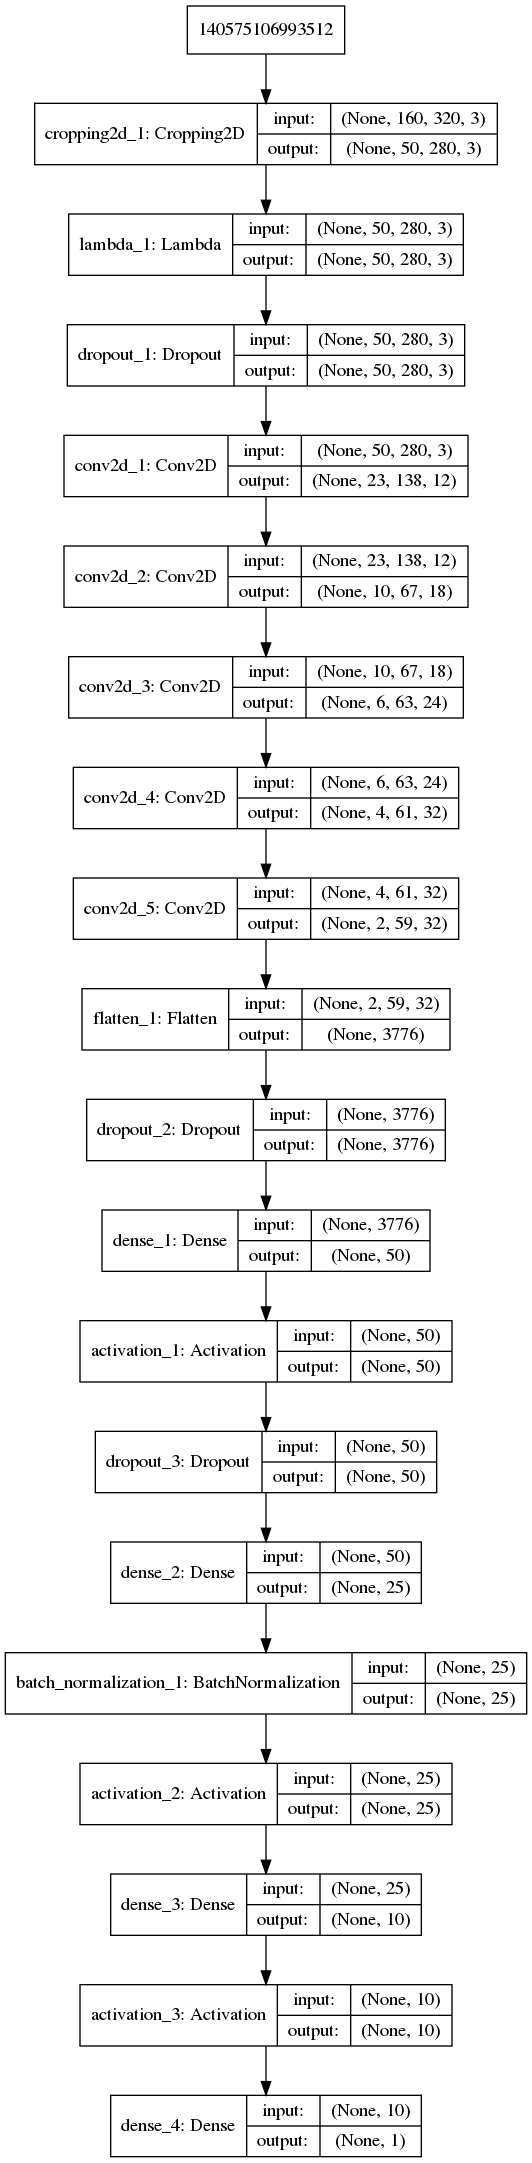
\includegraphics[width=0.3\linewidth]{writeup_figures/nvidia_reduced_model_structure}
		\caption{Model structure: Left, Nvidia's network, center, Lenet's network and right, reduced version of Nvidia's network.}
		\label{fig:models}
	\end{figure}



\begin{table}[H]
	\centering
	\begin{tabular}{|c|c|c|c|}
		\hline 
		&Nvidia  &Lenet  &Reduced Nvidia  \\ 
		\hline 
		Total params &   510,644& 1,495,449 & 223,842 \\ 
		\hline 
		Trainable params & 510,594 & 1,471,513 & 223,792\\ 
		\hline 
		Time per first epoch &  440 s& 250 s & 190 s\\ 
		\hline 
		Typical time per epoch & 180 s & 150-250 s & 200 s\\ 
		\hline 
		Number of epoch& 6 & 6  & 9 \\ 
		\hline 
	\end{tabular}
	\caption{Model structure.}
	\label{fig:table1}
\end{table}


\begin{figure}[H]
	\centering
	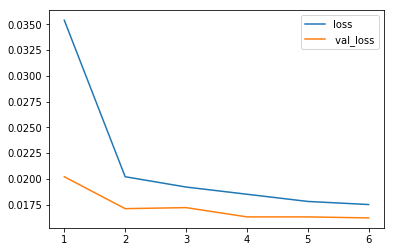
\includegraphics[width=0.3\linewidth]{writeup_figures/nvidia_loss}
	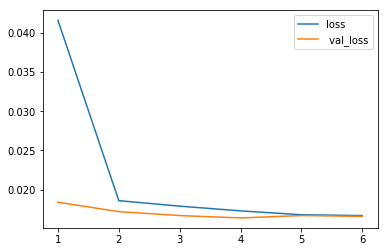
\includegraphics[width=0.3\linewidth]{writeup_figures/lenet_loss}		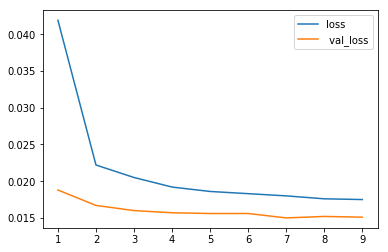
\includegraphics[width=0.3\linewidth]{writeup_figures/nvidia_reduced_loss}
	\caption{Convergence history: Left, Nvidia's network, center, Lenet's network and right, reduced version of Nvidia's network.}
	\label{fig:models}
\end{figure}

\begin{tabular}{|c|c|c|c|}
	\hline 
	Speed &Nvidia  &Lenet  &Reduced Nvidia  \\ 
	\hline 
	9 MPH  &   OK& OK & OK \\ 
	\hline 
	20 MPH& OK & Touches lane borders & Touches lane borders\\ 
	\hline 
	30 MPH&  OK& Passes lane borders & Drives out from track\\ 
	\hline  
\end{tabular} 


\end{document}